\section{BA ĐƯỜNG CONIC}
\subsection{LÝ THUYẾT CẦN NHỚ}
\subsubsection{Elip}
\begin{itemize}
	\item [\iconMT] \indam{Định nghĩa:} Cho hai điểm phân biệt $F_1$ và $F_2$. Đặt $F_1F_2=2c>0$. Tập hợp tất cả điểm $M$ thỏa $MF_1+MF_2=2a$, với $a>c>0$ là một elip.
	\item [\iconMT] \indam{Phương trình elip:} Trong mặt phẳng $Oxy$, cho hai điểm $F_1(-c;0)$,  $F_2(c;0)$ (hai tiêu điểm thuộc trục hoành). Với $b^2=a^2-c^2$, ta có phương trình elip có dạng \boxmini{$\dfrac{x^2}{a^2}+\dfrac{y^2}{b^2}=1$, với $a>b>0$.}
	\vspace{-0.8cm}
	\immini{
		\item [\iconMT] \indam{Hình dạng elip và các đại lượng liên quan:}\\
		\begin{tcolorbox}[colframe=orange,colback=orange!3,boxrule=0.2mm]
			\begin{itemize}
				\item Trục lớn $A_1A_2=2a$; Trục bé $B_1B_2=2b$;
				\item Tiêu cự $F_1F_2=2c$ và $a^2=b^2+c^2$.
				\item Tọa độ các đỉnh $A_1(-a;0)$, $A_2(a;0)$, $B_1(0;-b)$, $B_2(0;b)$.
				\item Tiêu điểm $F_1(-c;0)$,  $F_2(c;0)$.
			\end{itemize}
		\end{tcolorbox}
	}{\vspace{0.8cm}
		\begin{tikzpicture}[smooth,samples=300,scale=0.9,>=stealth,font=\footnotesize]
			\draw[->] (-3,0)--(3.2,0) node[below]{$x$};
			\draw[->] (0,-2)--(0,2.5) node[right]{$y$};
			\draw (0,0) node[below left]{$O$};
			\tkzDefPoints{0/0/O,-2.5/0/A_1,2.5/0/A_2,0/-1.5/B_1,0/1.5/B_2,-2/0/F_1,2/0/F_2}
			\draw[color=blue,thick] (O) ellipse (2.5cm and 1.5cm);
			\coordinate (M) at ($(O)+(60:2.5cm and 1.5cm)$);
			\tkzDrawPoints[size=3,fill=black](A_1,A_2,B_1,B_2,F_1,F_2,M)
			\tkzDrawSegments[dashed](M,F_1 M,F_2)
			\tkzLabelPoints[below right,font=\footnotesize](B_1)
			\tkzLabelPoints[above right,font=\footnotesize](B_2,A_2,M)
			\tkzLabelPoints[below ,font=\footnotesize](F_1,F_2)
			\tkzLabelPoints[above left,font=\footnotesize](A_1)
	\end{tikzpicture}}
\end{itemize}
\subsubsection{Hypebol}
\begin{itemize}
	\item [\iconMT] \indam{Định nghĩa:} Cho hai điểm phân biệt $F_1$ và $F_2$. Đặt $F_1F_2=2c>0$.Tập hợp tất cả điểm $M$ thỏa $\big|MF_1-MF_2\big|=2a$, với $0<a<c$ là một hypebol.
	\item [\iconMT] \indam{Phương trình hypebol:} Trong mặt phẳng $Oxy$, cho hai điểm $F_1(-c;0)$,  $F_2(c;0)$ (hai tiêu điểm thuộc trục hoành). Với $b^2=c^2-a^2$, ta có phương trình hyperbol có dạng \boxmini{$\dfrac{x^2}{a^2}-\dfrac{y^2}{b^2}=1$, với $a,b>0$.}
	\vspace{-0.8cm}
	\immini{
		\item [\iconMT] \indam{Hình dạng hypebol và các đại lượng liên quan:}\\
		\begin{tcolorbox}[colframe=orange,colback=orange!3,boxrule=0.2mm]
			\begin{itemize}
				\item Đoạn thẳng $A_1A_2=2a$ gọi là \textbf{trục thực}, đoạn thẳng $B_1B_2=2b$ gọi là \textbf{trục ảo} của hypebol.
				\item Tiêu cự $F_1F_2=2c$ và $a^2+b^2=c^2$.
				\item Tọa độ các đỉnh $A_1(-a;0)$, $A_2(a;0)$.
				\item Tiêu điểm $F_1(-c;0)$,  $F_2(c;0)$.
				\item Giao điểm $O$ của hai trục là \textbf{tâm đối xứng} của hypebol.
			\end{itemize}
		\end{tcolorbox}
	}{\vspace{0.8cm}
		\begin{tikzpicture}[scale=1, font=\footnotesize, line join=round, line cap=round, >=stealth]
			\def\a{1.2};
			\def\b{1};
			\pgfmathsetmacro\c{sqrt((\a)^2+(\b)^2)};
			\draw[->] ($(-{\a},0)-(1.5,0)$)--($({\a},0)+(1.5,0)$) node[above]{$x$};
			\draw[->] ($(0,-{\b})-(0,1)$)--($(0,{\b})+(0,1)$) node[left]{$y$};
			\draw[thick,blue,name path=h1,smooth, samples=200, domain=\a:2.5] plot (\x,{((\b)/(\a))*sqrt((\x)^2-(\a)^2)});
			\draw[thick,blue,yscale=-1,name path=h2,smooth, samples=200, domain=\a:2.5] plot (\x,{((\b)/(\a))*sqrt((\x)^2-(\a)^2)});
			\draw[thick,blue,xscale=-1,name path=h2,smooth, samples=200, domain=\a:2.5] plot (\x,{((\b)/(\a))*sqrt((\x)^2-(\a)^2)});
			\draw[thick,blue,xscale=-1,yscale=-1,name path=h2,smooth, samples=200, domain=\a:2.5] plot (\x,{((\b)/(\a))*sqrt((\x)^2-(\a)^2)});
			%			\def\xm{2};
			%			\pgfmathsetmacro\ym{((\b)/(\a))*sqrt((\xm)^2-(\a)^2)};
			\path
			(0,0) coordinate (O)
			(-\c,0) coordinate (F_1)
			(\c,0) coordinate (F_2)
			(-\a,0) coordinate (A_1)
			(\a,0) coordinate (A_2)
			(0,-\b) coordinate (B_1)
			(0,\b) coordinate (B_2)
			%				(\xm,\ym) coordinate (M)
			(\a,\b) coordinate (P)
			;
			\draw[fill=black] (O) circle(1pt)++(-0.15,-0.3) node{$O$};
			\draw[fill=black] (F_1) circle(1pt) node[below]{$F_1$};
			\draw[fill=black] (F_2) circle(1pt) node[below]{$F_2$};
			%			\draw[fill=black] (M) circle(1pt) node[right]{$M(x;y)$};
			\draw[fill=black] (A_1) circle(1pt) node[below right]{$A_1$};
			\draw[fill=black] (A_2) circle(1pt) node[below left]{$A_2$};
			\draw[fill=black] (B_1) circle(1pt) node[below right]{$B_1$};
			\draw[fill=black] (B_2) circle(1pt) node[above right]{$B_2$};
			\draw[fill=black] (P) circle(1pt) node[above]{$P$};
			\draw[dashed] (A_1)|-(B_1)-|(A_2)|-(B_2)-|(A_1);
			\draw [dashed,smooth,samples=200, domain=-2.3:2.3] plot (\x,{((\b)/(\a)*(\x))});
			\draw [dashed,smooth,samples=200, domain=-2.3:2.3] plot (\x,{-((\b)/(\a)*(\x))});
	\end{tikzpicture}}
\end{itemize}
\subsubsection{Parabol}
\begin{itemize}
	\immini{\item [\iconMT] \indam{Định nghĩa:} Cho một điểm $F$ và một đường thẳng $\Delta$ cố định không đi qua $F$. Tập hợp các điểm $M$ cách đều $F$ và $\Delta$ là một đường parabol. Điểm $F$ gọi là \textbf{tiêu điểm} và $\Delta$ gọi là \textbf{đường chuẩn} của parabol $(P)$.
		\boxmini{$MF=\mathrm{d}(M,\Delta)$}
		\item [\iconMT] \indam{Phương trình parabol:} Gọi $H$ là hình chiếu vuông góc của $F$ trên $\Delta$. Gọi khoảng cách từ tiêu điểm đến đường chuẩn là $p=HF$.
		Chọn hệ trục toạ độ $O x y$, với $O$ là trung điểm $HF$ (như hình vẽ) thì $F\left(\dfrac{p}{2} ; 0\right)$ và $\Delta: x=-\dfrac{p}{2}$. Khi đó, phương trình $(P)$ là \boxmini{$y^2=2px$, với $p>0$}}{
		\begin{tikzpicture}[scale=1.1, font=\footnotesize, line join=round, line cap=round, >=stealth]
			\def\xm{-1.3};
			\pgfmathsetmacro\ym{0.5*(\xm)^2};
			\path
			(0,0) coordinate (O)
			(0.5,0) coordinate (F)
			(\xm,\ym) coordinate (N)
			(\ym,-\xm) coordinate (M)
			;
			\draw[->] (-1.5,0)--(2.5,0) node[above]{$x$};
			\draw[->] (0,-2)--(0,2) node[right]{$y$};
			\draw[rotate=-90,smooth, samples=200, domain=-2:2,thick,blue] plot (\x,{0.5*(\x)^2});
			\draw (-0.5,2)--(-0.5,-2) node[left]{$\Delta$};
			\draw[fill=black] (O) circle(1pt)++(-0.2,-0.2) node{$O$};
			\draw[fill=black] (F) circle(1pt) +(0.5,-0.4) node{$F\left(\dfrac{p}{2};0\right)$};
			\draw[fill=black] (M) circle(1pt) node[right]{$M$};
			\draw (F)--(M)--(-0.5,-\xm);
			\draw ($(-0.5,-\xm)+(0.2,0)$)|-($(-0.5,-\xm)+(0,-0.2)$);
			\draw[fill=black] (-0.5,0) circle(1pt) node[below left]{$H$};
		\end{tikzpicture}
	}
	\item [\iconMT] \indam{Hình dạng parabol và các đại lượng liên quan:}
	\begin{tcolorbox}[colframe=orange,colback=orange!3,boxrule=0.2mm]
		\begin{itemize}
			\item $O$ là đỉnh; $Ox$ gọi là \textbf{trục đối xứng} của parabol $(P)$.
			\item $p$ gọi là \textbf{tham số tiêu} của parabol $(P)$.
			\item Tiêu điểm $F\left(\dfrac{p}{2} ; 0\right)$ và đường chuẩn $\Delta: x=-\dfrac{p}{2}$.
		\end{itemize}
	\end{tcolorbox}
\end{itemize}

\subsection{PHÂN LOẠI VÀ PHƯƠNG PHÁP GIẢI TOÁN}

\begin{dang}{Phương trình đường elip}
	\begin{itemize}
		\item [\iconMT] Xác định các yếu tố của elip $(E)$ có phương trình $\dfrac{x^2}{a^2}+\dfrac{y^2}{b^2}=1$, với $a>b>0$.
		\begin{itemize}
			\item Tính $c^2 = a^2 - b^2$.
			\item Độ dài trục lớn: $A_1 A_2 = 2a$, độ dài trục nhỏ: $B_1 B_2 = 2b$. Độ dài tiêu cự: $F_1 F_2 = 2c$.
			\item Tọa độ các đỉnh $A_1(-a;0)$, $A_2(a;0)$, $B_1(0;-b)$, $B_2(0;b)$.
			\item Tiêu điểm $F_1(-c;0)$,  $F_2(c;0)$.
		\end{itemize}
		\item [\iconMT] Viết phương trình $(E)$, ta thực hiện các bước:
		\begin{itemize}
			\item Từ dữ kiện bài toán, giải tìm $a$ và $b$,với $a>b>0$. 
			\item Ráp vào công thức $(E): \dfrac{x^{2}}{a^{2}}+\dfrac{y^{2}}{b^{2}}=1$.
		\end{itemize}
	\end{itemize}
\end{dang}

\begin{vd}
	Xác định tọa độ các đỉnh và độ dài các trục của các elip có phương trình sau:
	\begin{tasks}(2)
		\task $\dfrac{x^2}{16}+\dfrac{y^2}{4}=1$
		\task $\dfrac{x^2}{4}+\dfrac{y^2}{3}=1$
		\task $x^2+4y^2=1$.
		\task $4x^2+25y^2=36$.
	\end{tasks}
	\loigiai{
		\begin{enumerate}[a)]
			\item 	Từ phương trình $\dfrac{x^2}{16}+\dfrac{y^2}{4}=1$ ta có: $a=4$, $b=2$.\\
			Các đỉnh: $A_1(-4;0)$, $A_2(4;0)$, $B_1(0;-2)$, $B_2(0;2)$.\\
			Độ dài trục lớn: $A_1 A_2 = 2a = 8$, $B_1 B_2 = 2b = 4$.
			\item Từ phương trình $\dfrac{x^2}{4}+\dfrac{y^2}{3}=1$ ta có: $a^2=4$, $b^2=3$, suy ra $c=1$.\\
			Các tiêu điểm: $F_1(-1;0)$, $F_2(1;0)$.\\
			Độ dài tiêu cự: $F_1 F_2 = 2c = 2$.
			\item 	Ta có $x^2+4y^2=1 \Leftrightarrow \dfrac{x^2}{1}+\dfrac{y^2}{\frac{1}{4}}=1$: $a=1$, $b=\dfrac{1}{2}$.\\
			Các đỉnh: $A_1(-1;0)$, $A_2(1;0)$, $B_1(0;-\dfrac{1}{2})$, $B_2(0;\dfrac{1}{2})$.\\
			Độ dài trục lớn: $A_1 A_2 = 2a = 2$, $B_1 B_2 = 2b = 1$.
			\item Ta có $4x^2+25y^2=36 \Leftrightarrow \dfrac{x^2}{9}+\dfrac{y^2}{\frac{36}{25}}=1$, suy ra: $a^2=9$, $b^2=\dfrac{36}{25} \Rightarrow c=\dfrac{3\sqrt{21}}{5}$.\\
			Các tiêu điểm: $F_1(-\dfrac{3\sqrt{21}}{5};0)$, $F_2(\dfrac{3\sqrt{21}}{5};0)$.\\
			Độ dài tiêu cự: $F_1 F_2 = 2c = \dfrac{6\sqrt{21}}{5}$.
		\end{enumerate}
	}
\end{vd}\dongcham{10}

\begin{vd}
	Cho elip $(E)$ có độ dài trục lớn bằng $10$, tỉ số giữa tiêu cự và độ dài trục lớn là $\dfrac{3}{5}$. 
	\begin{tasks}(1)
		\task Tính độ dài trục nhỏ và viết phương trình chính tắc của elip.
		\task Tìm những điểm thuộc $(E)$ biết tung độ của chúng bằng $\sqrt{15}$.
	\end{tasks}
	
	\loigiai{
		Ta có $2a=10 \Rightarrow a=5$. Mà $\dfrac{c}{a}=\dfrac{3}{5} \Rightarrow c=3$.\\
		Do đó $b^2=a^2-c^2=16 \Rightarrow b=4$.
		\begin{itemize}
			\item [$\bullet$] Độ dài tục nhỏ $2b=8$.
			\item [$\bullet$] $(E) \colon \dfrac{x^2}{25}+\dfrac{y^2}{16}=1$.
		\end{itemize}
	}
\end{vd}\dongcham{10}

\begin{vd}
	Lập phương trình chính tắc của elip $(E)$, biết
	\begin{tasks}(1)
		\task độ dài trục lớn bằng  $6$, độ dài trục nhỏ bằng $4$.
		\task độ dài trục lớn bằng $10$, tiêu cự có độ dài bằng $6$.
		\task elip đi qua hai điểm $M(1;0), N(\dfrac{\sqrt{3}}{2};1).$
	\end{tasks}
	\loigiai{
		\begin{enumerate}[a)]
			\item Giả sử phương trình elip có dạng $(E): \dfrac{x^{2}}{a^{2}}+\dfrac{y^{2}}{b^{2}}=1$.\\Độ đài trục lớn bằng $6\Rightarrow 2a=6\Rightarrow a=3$.\\Độ dài trục nhỏ bằng $4\Rightarrow 2b=4\Rightarrow b=2.$\\Vậy phương trình elip là $\dfrac{x^{2}}{9}+\dfrac{y^{2}}{4}=1$. 
			\item Giả sử phương trình elip có dạng $(E): \dfrac{x^{2}}{a^{2}}+\dfrac{y^{2}}{b^{2}}=1$.\\
			Độ dài trục lớn bằng $10\Rightarrow 2a=10\Rightarrow a=5.$\\
			Độ dài tiêu cự bằng $6\Rightarrow 2c=6\Rightarrow c=3.$\\
			Ta có $b^{2}=a^{2}-c^{2}\Rightarrow b=4$.\\
			Vậy phương trình elip có dạng $\dfrac{x^{2}}{25}+\dfrac{y^{2}}{16}=1.$ 
			\item Giả sử phương trình elip có dạng $(E): \dfrac{x^{2}}{a^{2}}+\dfrac{y^{2}}{b^{2}}=1 $.\\
			Điểm $M\in (E)\Rightarrow \dfrac{1}{a^{2}}=1\Rightarrow a=1.$\\
			Điểm $N\in(E)\Rightarrow \dfrac{3}{4}+\dfrac{1}{b^{2}}=1\Rightarrow b=2.$\\
			Vậy phương trình chính tắc của elip có dạng $\dfrac{x^{2}}{1}+\dfrac{y^{2}}{4}=1 $.
	\end{enumerate} }   
\end{vd}\dongcham{10}

\begin{vd}
	\immini{
		Một mái vòm nhà hát có mặt cắt là hình nửa elip. Cho biết khoảng cách giữa hai tiêu điểm là $F'F=50\mathrm{m}$ và chiều dài của đường đi của một tia sáng từ $F'$ đến mái vòm rồi phản chiếu về $F$ là $100\mathrm{m}$. Viết phương trình chính tắc của elip đó.
	}{
		\begin{tikzpicture}[domain=0:4,line join = round, line cap = round,>=stealth,scale=0.7]
			\draw[->] (-5.5,0) -- (5.5,0) node[right] {$x$};
			\draw[->] (0,0) -- (0,4.5) node[above] {$y$};
			\draw (180:5 and 4) arc (180:0:5 and 4);
			\coordinate (I1) at ($(-2,0)!0.5!(135:5 and 4)$);
			\coordinate (J1) at ($(2,0)!0.5!(135:5 and 4)$);
			\draw[->] (-2,0) -- (I1);\draw[->](135:5 and 4)--(J1);
			\draw (-2,0) node[below]{$F$} -- (135:5 and 4)--(2,0)node[below]{$F'$};
			\draw (-2,0) -- (45:5 and 4)--(2,0);
			\draw (-2,0) -- (60:5 and 4)--(2,0);
			\draw (-2,0) -- (90:5 and 4)--(2,0);
			\draw (-2,0) -- (120:5 and 4)--(2,0);
			\coordinate (I3) at ($(-2,0)!0.5!(45:5 and 4)$);
			\coordinate (J3) at ($(2,0)!0.5!(45:5 and 4)$);
			\draw[->] (-2,0) -- (I3);\draw[->](45:5 and 4)--(J3);
			\coordinate (I4) at ($(-2,0)!0.5!(60:5 and 4)$);
			\coordinate (J4) at ($(2,0)!0.5!(60:5 and 4)$);
			\draw[->] (-2,0) -- (I4);\draw[->](60:5 and 4)--(J4);
			\coordinate (I5) at ($(-2,0)!0.5!(90:5 and 4)$);
			\coordinate (J5) at ($(2,0)!0.5!(90:5 and 4)$);
			\draw[->] (-2,0) -- (I5);\draw[->](90:5 and 4)--(J5);
			\coordinate (I6) at ($(-2,0)!0.5!(120:5 and 4)$);
			\coordinate (J6) at ($(2,0)!0.5!(120:5 and 4)$);
			\draw[->] (-2,0) -- (I6);\draw[->](120:5 and 4)--(J6);
			
		\end{tikzpicture}
	}
	\loigiai{
		Ta có $F'F=2c=50$, suy ra $c=25$.\\
		Tổng khoảng cách $F'M+FM=2a=100$, suy ra $a=50$.\\
		Ta có $b^2=a^2-c^2=50^2-25^2=1875$.\\
		Vậy elip có phương trình $\dfrac{x^2}{2500}+\dfrac{y^2}{1875}=1$.
		
	}
\end{vd}
\dongcham{3}

\begin{dang}{Phương trình đường hypebol}
	\begin{itemize}
		\item [\iconMT] Xác định các yếu tố của hypebol $(H)$ có phương trình $\dfrac{x^2}{a^2}-\dfrac{y^2}{b^2}=1$, với $a,b>0$.
		\begin{itemize}
			\item Tính $c^2 = a^2 + b^2$.
			\item Độ dài trục thực: $A_1 A_2 = 2a$, độ dài trục ảo: $B_1 B_2 = 2b$. Độ dài tiêu cự: $F_1 F_2 = 2c$.
			\item Tọa độ các đỉnh $A_1(-a;0)$, $A_2(a;0)$.
			\item Tiêu điểm $F_1(-c;0)$,  $F_2(c;0)$.
		\end{itemize}
		\item [\iconMT] Viết phương trình $(H)$, ta thực hiện các bước:
		\begin{itemize}
			\item Từ dữ kiện bài toán, giải tìm $a$ và $b$,với $a, b>0$. 
			\item Ráp vào công thức $(H): \dfrac{x^{2}}{a^{2}}-\dfrac{y^{2}}{b^{2}}=1$.
		\end{itemize}
	\end{itemize}
\end{dang}

\begin{vd}
	Xác định các tọa độ tiêu điểm, các đỉnh, độ dài trục thực, độ dài trục ảo và tiêu cự của hypebol $(H)$ có phương trình như sau:
	\begin{enumEX}[a)]{3}
		\item $(H): \dfrac{x^2}{16}-\dfrac{y^2}{4}=1$
		\item $(H): \dfrac{x^2}{8}-\dfrac{y^2}{4}=1$
		\item $(H): 4x^2-y^2=4$.
		\item $(H): 9x^2-25y^2=1$.
		\item $(H): 25x^2-16y^2=400$.
		\item $(H): 16x^2-9y^2=16$.
	\end{enumEX}
	\loigiai{}
\end{vd}\dongcham{11}

\begin{vd}
	Cho hyperbol $(H): \dfrac{x^2}{16}-\dfrac{y^2}{9}=1$.
	\begin{tasks}(1)
		\task Tìm độ dài trục ảo, trục thực, tiêu cự của $(H)$.
		\task Tìm điểm thuộc $(H)$ biết hoành độ của chúng bằng $\sqrt{7}$.
		\task Tìm trên $(H)$ những điểm $M(x;y)$ sao cho $MF_1 \perp MF_2$, với $F_1$, $F_2$ là hai tiêu điểm của $(H)$.
	\end{tasks}
	\loigiai{}
\end{vd}\dongcham{14}

\begin{vd}
	Lập phương trình chính tắc của hypebol, biết
	\begin{tasks}(2)
		\task Độ dài trục thực bằng 10 , trục ảo bằng 6.
		\task Độ dài trục thực bằng 8, tiêu cự bằng 10.
		\task Có một tiêu điểm $\mathrm{F}_2(5 ; 0)$ và đỉnh $\mathrm{A}_1(-4 ; 0)$.
		\task qua điểm $M(3 \sqrt{2} ;-4)$ và có một tiêu điểm là $F_2(5 ; 0)$.
	\end{tasks}
	\loigiai{
		\begin{enumEX}[a)]{1}
			\item 
			\item 
			\item 
			\item Phương trình chính tắc của $(H)$ có dạng $\frac{x^2}{a^2}-\frac{y^2}{b^2}=1$, trong đó $a, b>0$.
			Do $(H)$ có một tiêu điểm là $F_2(5 ; 0)$ nên ta có
			$$
			c=5 \Rightarrow a^2+b^2=c^2=25 \Leftrightarrow a^2=25-b^2 .
			$$
			Vì $(H)$ đi qua điểm $M(3 \sqrt{2} ; 4)$ nên ta có
			$$
			\frac{(3 \sqrt{2})^2}{a^2}-\frac{4^2}{b^2}=1 \Leftrightarrow \frac{18}{a^2}-\frac{16}{b^2}=1 .
			$$
			Đặt $t=b^2>0 \Rightarrow a^2=25-t$. Thay vào (1) ta được
			$$
			\begin{aligned}
				\frac{18}{25-t}-\frac{16}{t}=1 & \Leftrightarrow 18 t-16(25-t)=(25-t) t \\
				& \Leftrightarrow t^2+9 t-400=0 \Leftrightarrow\left[\begin{array}{l}
					t=16 \\
					t=-25 .
				\end{array}\right.
			\end{aligned}
			$$
			Đối chiếu với điều kiện $t>0$ ta được $t=16$.
			Suy ra $b^2=t=16, a^2=25-t=9$.
			Vậy phương trình chính tắc của $(H)$ là $\frac{x^2}{9}-\frac{y^2}{16}=1$.
			\begin{note}
				Trong phương trình chính tắc của hypebol, ta có $0<a, b<c$. Ngoài ra không có sự so sánh giữa $a$ và $b$.
			\end{note}
	\end{enumEX}}
\end{vd}\dongcham{15}
\begin{vd}
	\immini{
		Một tháp triển lãm có mặt cắt hình hypebol có phương trình $$\dfrac{x^2}{18^2}-\dfrac{y^2}{36^2}=1$$
		Cho biết chiều cao của tháp là $100\,\mathrm{m}$ và khoảng cách từ nóc tháp đến tâm đối xứng của hypebol bằng khoảng cách từ tâm đối xứng đến đáy. Tính bán kính nóc và bán kính đáy của tháp.
	}{
		\begin{tikzpicture}[line join = round, line cap = round,>=stealth,scale=1]
			\draw[->] (-2,0) -- (2,0) node[right] {$x$};
			\draw[->] (0,-3) -- (0,3.2) node[above] {$y$};
			\draw[domain=-2:2,smooth, samples=150] plot ({(0.35*(\x))^(2)+0.5},\x);
			\draw[domain=-2:2,smooth, samples=150] plot (-{(0.35*(\x))^(2)-0.5},\x);
			\draw (0,2.05) ellipse (1 and 0.4);
			\draw[dashed] (0,-2.05) ellipse (1 and 0.4);
			\draw (0,-2.05)+(0:1 and 0.4) arc (0:-180:1 and 0.4);
			\fill (0,0)node[above right]{$O$} circle (1pt);
		\end{tikzpicture}
	}
	\loigiai{
		Do tính đối xứng của hypebol nên ta có hai bán kính của nóc và đáy tháp đều bằng $r$.\\
		Do điểm $M(r;50)$ nằm trên hypebol nên thay tọa độ của điểm $M$ vào phương trình của hypebol ta có:\\ $\dfrac{r^2}{18^2}-\dfrac{50^2}{36^2}=1 \Rightarrow r=18\sqrt{1+\dfrac{50^2}{36^2}} \approx 31(\mathrm{m})$.\\
		Vậy bán kính của nóc và đáy của tháp bằng $31\,\mathrm{m}$.
	}
\end{vd}\dongcham{10}

\begin{dang}{Phương trình đường parabol}
	\begin{itemize}
		\item [\iconMT] Xác định các yếu tố của parabol $(P)$ có phương trình $y^2=2px$, với $p>0$.
		\begin{itemize}
			\item $p$ gọi là \textbf{tham số tiêu} của parabol $(P)$.
			\item Tiêu điểm $F\left(\dfrac{p}{2} ; 0\right)$ và đường chuẩn $\Delta: x=-\dfrac{p}{2}$.
		\end{itemize}
		\item [\iconMT] Viết phương trình chính tắc của $(P)$, ta thực hiện các bước:
		\begin{itemize}
			\item Từ dữ kiện bài toán, giải tìm $p>0$. 
			\item Ráp vào công thức $(P): y^2=2px$.
		\end{itemize}
	\end{itemize}
\end{dang}

\begin{vd}
	Tìm tọa độ tiêu điểm, phương trình đường chuẩn của các parabol $(P)$ có phương trình chính tắc như sau:
	\begin{enumEX}[a)]{3}
		\item $(P) \colon y^2=2x$.
		\item $(P) \colon y^2=4x$.
		\item $(P) \colon y^2=x$.
		\item $(P) \colon y^2=9x$.
		\item $(P) \colon y^2-6x=0$.
		\item $(P) \colon 2y^2-4x=0$.
	\end{enumEX}
	\loigiai{}
\end{vd}\dongcham{20}
\begin{vd}
	Lập phương trình chính tắc của parabol $(P)$ biết
	\begin{enumEX}[a)]{2}
		\item $(P)$ có tiêu điểm $F(3 ; 0)$.
		\item $(P)$ có tiêu điểm $F(1 ; 0)$.
		\item $(P)$ đi qua điểm $M(6 ;-2)$.
		\item $(P)$ đi qua điểm $M(1 ;-4)$.
		\item $(P)$ có đường chuẩn $x=-3$.
		\item $(P)$ có đường chuẩn $x+2=0$.
	\end{enumEX}
	\loigiai{}
\end{vd}\dongcham{19}

\begin{vd}%[0H3K5-4]
	\immini{Một chiếc đèn có mặt cắt ngang là hình parabol như hình bên. Hình parabol có chiều rộng giữa hai mép vành là $AB=40$cm và chiều sâu $h=30$cm ($h$ bằng khoảng cách từ $O$ đến $AB$). Bóng đèn nằm ở tiêu điểm $S$. Viết phương trình chính tắc của parabol đó.}
	{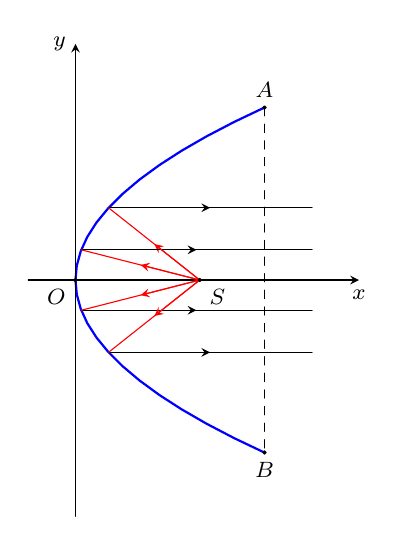
\begin{tikzpicture}[scale=0.6, font=\footnotesize, line join=round, line cap=round, >=stealth]
			
			\draw[domain=-3.65:3.65, blue,thick] plot({3/10*(\x)^2},\x);
			%\draw[gray!10] (-1,-1) grid (5,5);
			\draw[->] (-1,0)--(6,0) node[below]{$x$};
			\draw[->] (0,-5)--(0,5) node[left]{$y$};
			\coordinate (A) at (4,3.65); 
			\coordinate (B) at (4,-3.65); 
			\coordinate (O) at (0,0); 
			\coordinate (C) at (0.12,0.64); 
			\coordinate (C') at (0.12,-0.64); 
			\coordinate (D) at (0.7,1.53); 
			\coordinate (D') at (0.7,-1.53); 
			\coordinate (F) at (5.01,1.53); 
			\coordinate (F') at (5.01,-1.53); 
			\coordinate (G) at (5.01,0.64); 
			\coordinate (G') at (5.01,-0.64); 
			\coordinate (E) at (2.63,0); 
			\coordinate (H1) at (1.67,0.76); 
			\coordinate (H2) at (1.67,-0.76); 
			\coordinate (H3) at (1.38,0.32); 
			\coordinate (H4) at (1.38,-0.32); 
			\coordinate (K1) at (2.85,1.53); 
			\coordinate (K2) at (2.85,-1.53); 
			\coordinate (K3) at (2.56,0.64); 
			\coordinate (K4) at (2.56,-0.64); 
			\draw  (F)--(D) (G)--(C) (F')--(D') (G')--(C') ;
			\draw[dashed] (A)--(B);
			\draw[red,->] (E)--(H1); 
			\draw[->] (D)--(K1) ;
			\draw[red,->] (E)--(H3); 
			\draw[->] (C)--(K3) ;
			\draw[red,->] (E)--(H4); 
			\draw[->] (C')--(K4) ;
			\draw[red,->] (E)--(H2); 
			\draw[->] (D')--(K2) ;
			
			\draw[red] (E)--(C) (E)--(D) (E)--(C') (E)--(D');
			
			\draw[fill=black] (A) circle (1pt) node [above] {$A$};
			\draw[fill=black] (B) circle (1pt) node [below] {$B$};
			\draw[fill=black] (E) circle (1pt) node [below right] {$S$};
			\draw[fill=black] (O) circle (1pt) node [below left] {$O$};
	\end{tikzpicture}}
	
	\loigiai{Gắn hình parabol vào hệ trục như đề bài, dựa vào giả thiết bài toán ta có tọa độ điểm $A(30;20)$. Parabol đi qua điểm $A$ nên ta có phương trình 
		\begin{eqnarray*}
			20^2=2p\cdot 30 \Leftrightarrow p=\dfrac{20}{3}.
		\end{eqnarray*}
		Vậy ta có phương trình chính tắc của parabol đó là $y^2=\dfrac{40x}{3}$.	
	}
\end{vd}\dongcham{10}

\subsection{BÀI TẬP TỰ LUYỆN}

\begin{baitap}
	Xác định tọa độ các đỉnh và các tiêu điểm của các elip có phương trình sau:
	\begin{tasks}(2)
		\task $\dfrac{x^2}{100} + \dfrac{y^2}{64} = 1$; 
		\task $\dfrac{x^2}{4} + y^2 = 1$;
		\task $16x^2+25y^2=1$;
		\task $0,25 x^2+9y^2=1$.
	\end{tasks}
	\loigiai{
		\begin{enumerate}[a)]
			\item Ta có $a^2=100, b^2=64 \Rightarrow a=10, b=8, c=6$.\\
			Vậy $A_1(-10;0)$, $A_2(10;0)$, $B_1(0;-8)$, $B_2(0;8), F_1(-6;0), F_2(6;0)$.
			\item Ta có $a^2=4, b^2=1 \Rightarrow a=2, b=1, c=\sqrt{3}$.\\
			Vậy $A_1(-2;0)$, $A_2(2;0)$, $B_1(0;-1)$, $B_2(0;1), F_1(-\sqrt{3};0), F_2(\sqrt{3};0)$.
			\item Ta có $16x^2+25y^2=1 \Leftrightarrow \dfrac{x^2}{\frac{1}{16}} + \dfrac{y^2}{\frac{1}{25}} = 1$.\\
			Do đó: $A_1(-\dfrac{1}{4};0)$, $A_2(\dfrac{1}{4};0)$, $B_1(0;-\dfrac{1}{5})$, $B_2(0;\dfrac{1}{5}), F_1(-\dfrac{3}{20};0), F_2(\dfrac{3}{20};0)$.
			\item Ta có $0,25 x^2+9y^2=1 \Leftrightarrow \dfrac{x^2}{4} + \dfrac{y^2}{\frac{1}{9}} = 1$.\\
			Vậy: $A_1(-\dfrac{1}{4};0)$, $A_2(\dfrac{1}{4};0)$, $B_1(0;-\dfrac{1}{5})$, $B_2(0;\dfrac{1}{5}), F_1(-\dfrac{3}{20};0), F_2(\dfrac{3}{20};0)$.
	\end{enumerate}}
\end{baitap}\cham{13}

\begin{baitap}%[0H3B4-1]
	Tìm tọa độ các tiêu điểm, tọa độ các đỉnh, độ dài trục thực và trục ảo của các hypebol sau
	\begin{listEX}[2]
		\item $\dfrac{x^2}{16}-\dfrac{y^2}{9}=1$;
		\item $\dfrac{x^2}{64}-\dfrac{y^2}{36}=1$;
		\item $x^2-16y^2=16$;
		\item $9x^2-16y^2=144$.
	\end{listEX}
	\loigiai{
		\begin{enumerate}
			\item Ta có $a^2=16\Rightarrow a=4$ và $b^2=9\Rightarrow b=3$.\\
			Suy ra $c=\sqrt{a^2+b^2}=\sqrt{16+9}=5$.\\
			Do đó
			\begin{itemize}
				\item Tọa độ các tiêu điểm là $F_1 (-5;0)$; $F_2 (5;0)$.
				\item Tọa độ các đỉnh là $A_1 (-4;0)$; $A_2 (4;0)$.
				\item Độ dài trục thực là $A_1 A_2=2a=8$.
				\item Độ dài trục ảo là $B_1 B_2=2b=6$.
			\end{itemize}
			\item Ta có $a^2=64\Rightarrow a=8$ và $b^2=36\Rightarrow b=6$.\\
			Suy ra $c=\sqrt{a^2+b^2}=\sqrt{64+36}=10$.\\
			Do đó
			\begin{itemize}
				\item Tọa độ các tiêu điểm là $F_1 (-10;0)$; $F_2 (10;0)$.
				\item Tọa độ các đỉnh là $A_1 (-8;0)$; $A_2 (8;0)$.
				\item Độ dài trục thực là $A_1 A_2=2a=16$.
				\item Độ dài trục ảo là $B_1 B_2=2b=12$.
			\end{itemize}
			\item Ta có $x^2-16y^2=16 \Leftrightarrow \dfrac{x^2}{16}-\dfrac{y^2}{1}=1$.
			Nên $a^2=16\Rightarrow a=4$ và $b^2=1\Rightarrow b=1$.\\
			Suy ra $c=\sqrt{a^2+b^2}=\sqrt{16+1}=\sqrt{17}$.\\
			Do đó
			\begin{itemize}
				\item Tọa độ các tiêu điểm là $F_1 \left(-\sqrt{17};0\right)$; $F_2 \left(\sqrt{17};0\right)$.
				\item Tọa độ các đỉnh là $A_1 (-4;0)$; $A_2 (4;0)$.
				\item Độ dài trục thực là $A_1 A_2=2a=8$.
				\item Độ dài trục ảo là $B_1 B_2=2b=2$.
			\end{itemize}
			\item Ta có $9x^2-16y^2=144 \Leftrightarrow \dfrac{x^2}{16}-\dfrac{y^2}{9}=1$.
			Nên $a^2=16\Rightarrow a=4$ và $b^2=9\Rightarrow b=3$.\\
			Suy ra $c=\sqrt{a^2+b^2}=\sqrt{16+9}=5$.\\
			Do đó
			\begin{itemize}
				\item Tọa độ các tiêu điểm là $F_1 (-5;0)$; $F_2 (5;0)$.
				\item Tọa độ các đỉnh là $A_1 (-4;0)$; $A_2 (4;0)$.
				\item Độ dài trục thực là $A_1 A_2=2a=8$.
				\item Độ dài trục ảo là $B_1 B_2=2b=6$.
			\end{itemize}
		\end{enumerate}
	}
\end{baitap}\cham{20}

\begin{baitap}%[Tex hóa SGK CD-CT,T7/22, Nguyễn Tiến]%[0H3B5-1]
	Tìm tọa độ tiêu điểm, phương trình đường chuẩn của các parabol sau
	\begin{listEX}[2]
		\item $y^2=12x$;
		\item $y^2=x$.
	\end{listEX}
	\loigiai{
		\begin{enumerate}
			\item Ta có $2p=12 \Leftrightarrow p=6$.\\
			Do đó
			\begin{itemize}
				\item Tọa độ tiêu điểm là $F(3;0)$.
				\item Phương trình đường chuẩn là $\Delta\colon x+3=0$.
			\end{itemize}
			\item Ta có $2p=1 \Leftrightarrow p=\dfrac{1}{2}$.\\
			Do đó
			\begin{itemize}
				\item Tọa độ tiêu điểm là $F\left(\dfrac{1}{4};0\right)$.
				\item Phương trình đường chuẩn là $\Delta\colon x+\dfrac{1}{4}=0$.
			\end{itemize}
		\end{enumerate}
	}
\end{baitap}\cham{7}

\begin{baitap}%[10EX- Tex hóa CD -CT-hk2-Thầy Trịnh Xuân]%[0H3B5-3]
	Viết phương trình chính tắc của:
	\begin{listEX}[1]%số cột
		\item Elip có trục lớn bằng $12$ và trục nhỏ bằng $8$;
		\item Hypebol có tiêu cự $2c=18$ và độ dài trục thực $2a=14$;
		\item Parabol có tiêu điểm $F(5;0)$.
	\end{listEX}
	\loigiai{
		\begin{listEX}[1]%số cột
			\item Ta có $2a=12$, $2b=8$ suy ra $a=6, b=4$. Vậy phương trình của Elip là $(E) \colon\dfrac{x^2}{36}+\dfrac{y^2}{16}=1$;
			\item Ta có $2c=18$, $2a=14$ suy ra $c=9, a=7$ nên\\
			$b^2=c^2-a^2 = 9^2 -7^2 = 32$. Vậy phương trình của Hypebol là $(H) \colon \dfrac{x^2}{49}-\dfrac{y^2}{32}=1$;
			\item Ta có $\dfrac{p}{2}=5$ nên $p=10$. Vậy phương trình của Parabol là $y^2 = 2px\Leftrightarrow (P) \colon y^2=20x$.
		\end{listEX}
	}
\end{baitap}\cham{14}


\begin{baitap}
	Cho parabol $(P): y^2=4 x$ và điểm $M\left(x_0 ; y_0\right) \in(P)$.
	\begin{tasks}(1)
		\task Tính khoảng cách từ $M$ đến tiêu điểm $F$.
		\task Tìm tọa độ của điểm $M$ biết $MF=2$.
		\task Đường thẳng $d$ qua $F$ cắt $(P)$ tại hai điểm $A$ và $B$. Chứng minh: $AB=x_A+x_B+2$.
	\end{tasks}
	\loigiai{}
\end{baitap}\cham{10}

\begin{baitap}
	Trong mặt phẳng $Oxy$, cho elip $(E): 9x^2+16y^2=144$. Tìm tất cả điểm $M$ thuộc elip sao cho góc $\widehat{F_1MF_2}$ bẳng $60^0$.
	\loigiai{
		Phương trình chính tắc của elip $(E): \dfrac{x^2}{16}+\dfrac{y^2}{9}=1$. Khi đó: $a=4, b=3, c=\sqrt{7}$.
		\\
		Gọi $M(x;y)$ là điểm cần tìm. Ta có:
		$$MF_1=4+\dfrac{\sqrt{7}}{4}x;\quad MF_2=4-\dfrac{\sqrt{7}}{4}x;\quad  F_1F_2=2\sqrt{7} $$
		Áp dụng định lí cosin trong tam giác $F_1MF_2$, ta  được:
		$$F_1F_2^2=MF_1^2+MF_2^2-2MF_1.MF_2.\cos \widehat{F_1MF_2}$$
		$$28 = 2\left(16+\dfrac{7}{16}x^2 \right) -\left( 4+\dfrac{\sqrt{7}}{4}x\right) \left( 4-\dfrac{\sqrt{7}}{4}x\right) \Leftrightarrow x^2 = \dfrac{64}{7}$$
		$$\Leftrightarrow  x= \dfrac{8}{\sqrt{7}} \text{ hoặc }  x=-\dfrac{8}{\sqrt{7}}.$$
		Vậy có $4$ điểm thỏa đề bài là $\left( \dfrac{8}{\sqrt{7}} ; \dfrac{3\sqrt{3}}{\sqrt{7}}\right) ; \left(- \dfrac{8}{\sqrt{7}} ; \dfrac{3\sqrt{3}}{\sqrt{7}}\right) ; \left( \dfrac{8}{\sqrt{7} };- \dfrac{3\sqrt{3}}{\sqrt{7}}\right) ; \left( -\dfrac{8}{\sqrt{7} };- \dfrac{3\sqrt{3}}{\sqrt{7}}\right) $.}
\end{baitap}\cham{15}

\begin{baitap}%[0H3T4-2]
	Một tháp làm nguội của một nhà máy có mặt cắt là hình hypebol có phương trình $\dfrac{x^2}{30^2}-\dfrac{y^2}{50^2}=1$. Biết chiều cao của tháp là $120\mathrm{m}$ và khoảng cách từ nóc tháp đến tâm đối xứng của hypebol bằng $\dfrac{1}{2}$ khoảng cách từ tâm đối xứng đến đáy. Tính bán kính nóc và bán kính đáy của tháp.
	\loigiai{
		\immini{
			Gọi $r$ và $R$ lần lượt là bán kính nóc và bán kính đáy của tháp. Ta tính được khoảng cách từ nóc tháp đến tâm
			đối xứng của hypebol bằng $40\mathrm{m}$ và khoảng cách từ tâm đối xứng đến đáy bằng $80\mathrm{m}$.\\
			Thay toạ độ hai điểm $M(R;-80)$ và $N(r;40)$ vào phương trình hypebol ta tính được:\\
			$R=30\sqrt{1+\dfrac{(-80)^2}{50^2}} \approx 57(m);r=30\sqrt{1+\dfrac{40^2}{50^2}} \approx 38(\mathrm{m})$.
			
		}{
			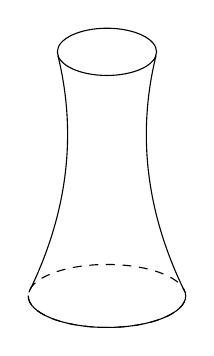
\begin{tikzpicture}[line join = round, line cap = round,>=stealth,scale=1]
				\draw[domain=-2:1,smooth, samples=150] plot ({(0.35*(\x))^(2)+0.5},\x);
				\draw[domain=-2:1,smooth, samples=150] plot (-{(0.35*(\x))^(2)-0.5},\x);
				\draw (0,1.05) ellipse (0.63 and 0.3);
				\draw[dashed] (0,-2.05) ellipse (1 and 0.4);
				\draw (0,-2.05)+(0:1 and 0.4) arc (0:-180:1 and 0.4);
			\end{tikzpicture}
		}
	}
\end{baitap}\cham{10}

\begin{baitap}%[0H3K3-2]
	Để cắt một bảng hiệu quảng cáo hình elip có trục lớn là $1\mathrm{m}$ và trục nhỏ là $0{,}6\mathrm{m}$ từ một tấm ván ép hình chữ nhật có kích thước $1\mathrm{m}\times 0{,}6\mathrm{m}$, người ta vẽ hình elip đó lên tấm ván ép như hướng dẫn sau:
	\immini{
		Chuẩn bị:\\
		- Hai cái đinh, một vòng dây kín không đàn hồi, bút chì.\\
		Thục hiện:\\
		- Xác định vị trí (hai tiêu điểm của elip) và ghim hai cái đinh lên hai điểm đó trên tấm ván.\\
		- Quàng vòng dây qua hai chiếc đinh và kéo căng tại một điểm $M$ nào đó. Tựa đầu bút chì vào trong\\
		vòng dây tại điểm $M$ rồi di chuyển sao cho dây luôn luôn căng. 
	}{
		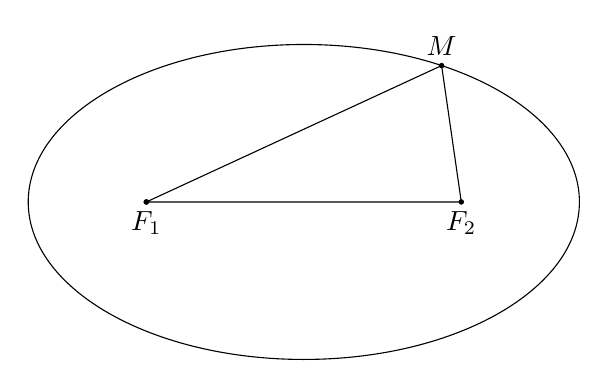
\begin{tikzpicture}[line join = round, line cap = round,>=stealth,scale=1]
			\draw (0,0) ellipse (3.5 and 2);
			\draw (-2,0)node[below]{$F_1$} -- (2,0)node[below]{$F_2$} -- (60:3.5 and 2)node[above]{$M$}--(-2,0);
			\fill (-2,0) circle (1pt);\fill (2,0) circle (1pt);\fill (-2,0) circle (1pt);\fill (60:3.5 and 2) circle (1pt);
		\end{tikzpicture}
	}
	Đầu bút chì vạch lên tấm bìa một đường mà ta gọi là đường elip. (Xem minh hoạ trong Hình bên). Phải ghim hai cái đỉnh cách các mép tấm ván ép bao nhiêu và lấy vòng dây có độ dài là bao nhiêu?
	\loigiai{
		Ta có $2a=1\mathrm{m}=100\mathrm{cm};2b=0{,}6\mathrm{m}=60\mathrm{cm}$.\\
		Suy ra $c^2=a^2-b^2=50^2-30^2=1600 \Rightarrow c=40$.\\
		Ta có $a-c=10(\mathrm{cm})$ và $2a+2c=180(\mathrm{cm})$.\\
		Vậy phải ghim hai cái đinh cách các mép tấm ván ép $10\rm{cm}$ và lấy vòng dây có độ dài là $180\mathrm{cm}$ hay $1,8\mathrm{m}$.
		
	}
\end{baitap}\cham{10}

\begin{baitap}%[0H3B3-4]
	\immini{
		Thang leo gợn sóng cho trẻ em trong công viên có hai khung thép cong hình nửa elip cao $100\rm{cm}$ và khoảng cách giữa hai chân là $240\rm{cm}$.
		\begin{listEX}[]%số cột
			\item Hãy chọn hệ toạ độ thích hợp và viết phương trình chính tắc của elip nói trên.
			\item Tính khoảng cách thẳng đứng từ một điểm cách chân khung $20\rm{cm}$ lên đến khung thép.	
		\end{listEX}
	}{
		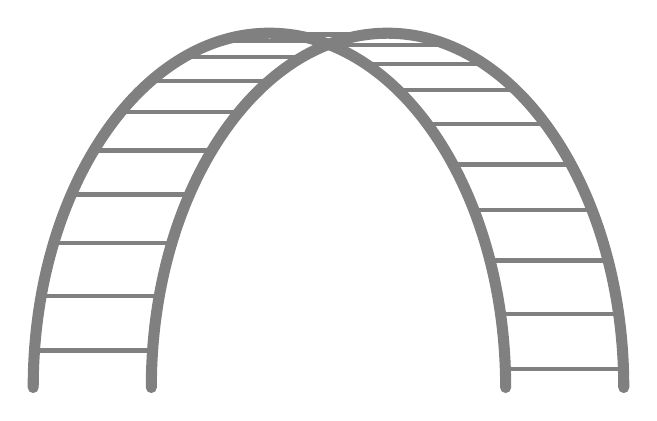
\begin{tikzpicture}[line join = round, line cap = round,>=stealth,scale=0.7]
			\tikzset{Thang-leo/.pic={
					\def\a{3}
					\def\b{1.5*\a}
					\def\d{1.5}
					\draw[gray,line width=4pt](\a,0)arc(0:180:{\a} and {\b});
					\draw[gray,line width=4pt,shift={(\d,0)}](\a,0)arc(0:180:{\a} and {\b});
					\foreach \g in{3,12,...,180}
					\draw[gray,line width=1.5pt](\g: {\a} and {\b})--++(0:\d);
			}}
			\path(0,0)pic{Thang-leo};
		\end{tikzpicture}
	}
	
	\loigiai{
		\begin{listEX}[1]%số cột
			\item Phương trình chính tắc của elip là $\dfrac{x^2}{120^2}+\dfrac{y^2}{100^2}=1$.
			\item Thay $x=120-20=100$ vào phương trình elip ta có:\\
			$\dfrac{100^2}{120^2}+\dfrac{y^2}{100^2}=1 \Rightarrow y^2=100^2\left(1-\dfrac{100^2}{120^2}\right) \Rightarrow y \approx 55(\rm{cm})$.
		\end{listEX}
	}
\end{baitap}\cham{9}

\begin{baitap}%[Tex hóa SGK CD,T93/104, Nguyễn Hoài Nam]%[0H3B3-4]
	\immini{Ta biết rằng Mặt Trăng chuyển động quanh Trái Đất theo quỹ đạo là một elip mà Trái Đất là một tiêu điểm. Elip đó có $A_1A_2=768800$ km và $B_1B_2=767619$ km (\textit{Nguồn: Ron Larson ($2014$), Precalculus Real Mathematics, Real People, Cengage}) (Hình minh họa). Viết phương trình chính tắc của elip đó.}
	{
		\begin{tikzpicture}[scale=0.7,>=stealth, font=\footnotesize, line join=round, line cap=round]
			\draw[->] (-4.5,0)--(4.5,0) node[below right] {$x$};
			\draw [->] (0,-2.5)--(0,2.5) node[above right] {$y$};
			\draw (-4,0) node[above left]{$A_1$} (4,0) node[above right] {$A_2$} (0,2) node[above left] {$B_2$} (0,-2) node[below left] {$B_1$} (0,0) node[below left] {$O$};
			\draw (0,0) ellipse (4cm and 2cm);
			\fill[color= green] (-1.5,0) circle (8pt);
			\fill[color=red] (1,1.94) circle (3pt) ;
			\node[above] at (-1.5,0.25) {Trái Đất} ;
			\node[above] at (1.2,1.9) {Mặt Trăng} ;
		\end{tikzpicture}
	}
	\loigiai{
		Phương trình chính tắc của elip có dạng: $\dfrac{x^2}{a^2}+\dfrac{y^2}{b^2}=1$, với $a>b>0$.\\
		Ta có $\heva{&A_1A_2=768800\\&B_1B_2=767619}\Leftrightarrow \heva{&2a=768800\\&2b=767619} \Leftrightarrow \heva{&a=384400\\&b=\dfrac{767619}{2}.}$\\
		Vậy phương trình chính tắc của elip là: $\dfrac{x^2}{384400^2}+\dfrac{4y^2}{767619^2}=1$.
	}
\end{baitap}\cham{10}



